\title{Risiko}

\section{Risk Analysis}

Risk analysis is an ongoing process that continuously evaluates risk throughout the project's lifecycle. It is the responsibility of the risk manager to ensure that this process takes place regularly and consistently during the project. This is crucial because it raises awareness among both us and our customers about potential risks and vulnerabilities, encourages necessary improvements, and facilitates necessary changes. Such analysis can help the risk manager identify new risks and changes that require attention along the way. \cite{Risk1}

After identifying risks, it is essential to prioritize them based on their probability and severity. Moreover, measures should be put in place to manage them effectively if they occur. While everyone on the team should participate in assessing the project's risks, the risk manager will be primarily responsible for ensuring quality assurance. \cite{Risk2}

A risk analysis was conducted for our project, wherein we identified both internal and external risks. Internal risks are linked with factors that are under our control, whereas external risks are associated with factors that lie beyond our control.\cite{RiskInternalExternal} A few examples of these risks are:\\



Internal risks:
\begin{itemize}
    \item If multiple get sick at the same time? 
    \item If someone suddenly wants to quit
\end{itemize}
External risks:
\begin{itemize}
    \item New nationwide pandemic
    \item Component availability with regard to a global shortage
\end{itemize}

After identifying the risks at this stage, we evaluate their potential consequences and determine the appropriate measures that can be taken if they occur. To gain a better overview, we record the risks in a table that includes a unique code, a description of the risk event, recommended measures, probability (P), consequence (C), and priority. Below is a comprehensive overview of both internal and external risks:


\begin{figure}
\centering
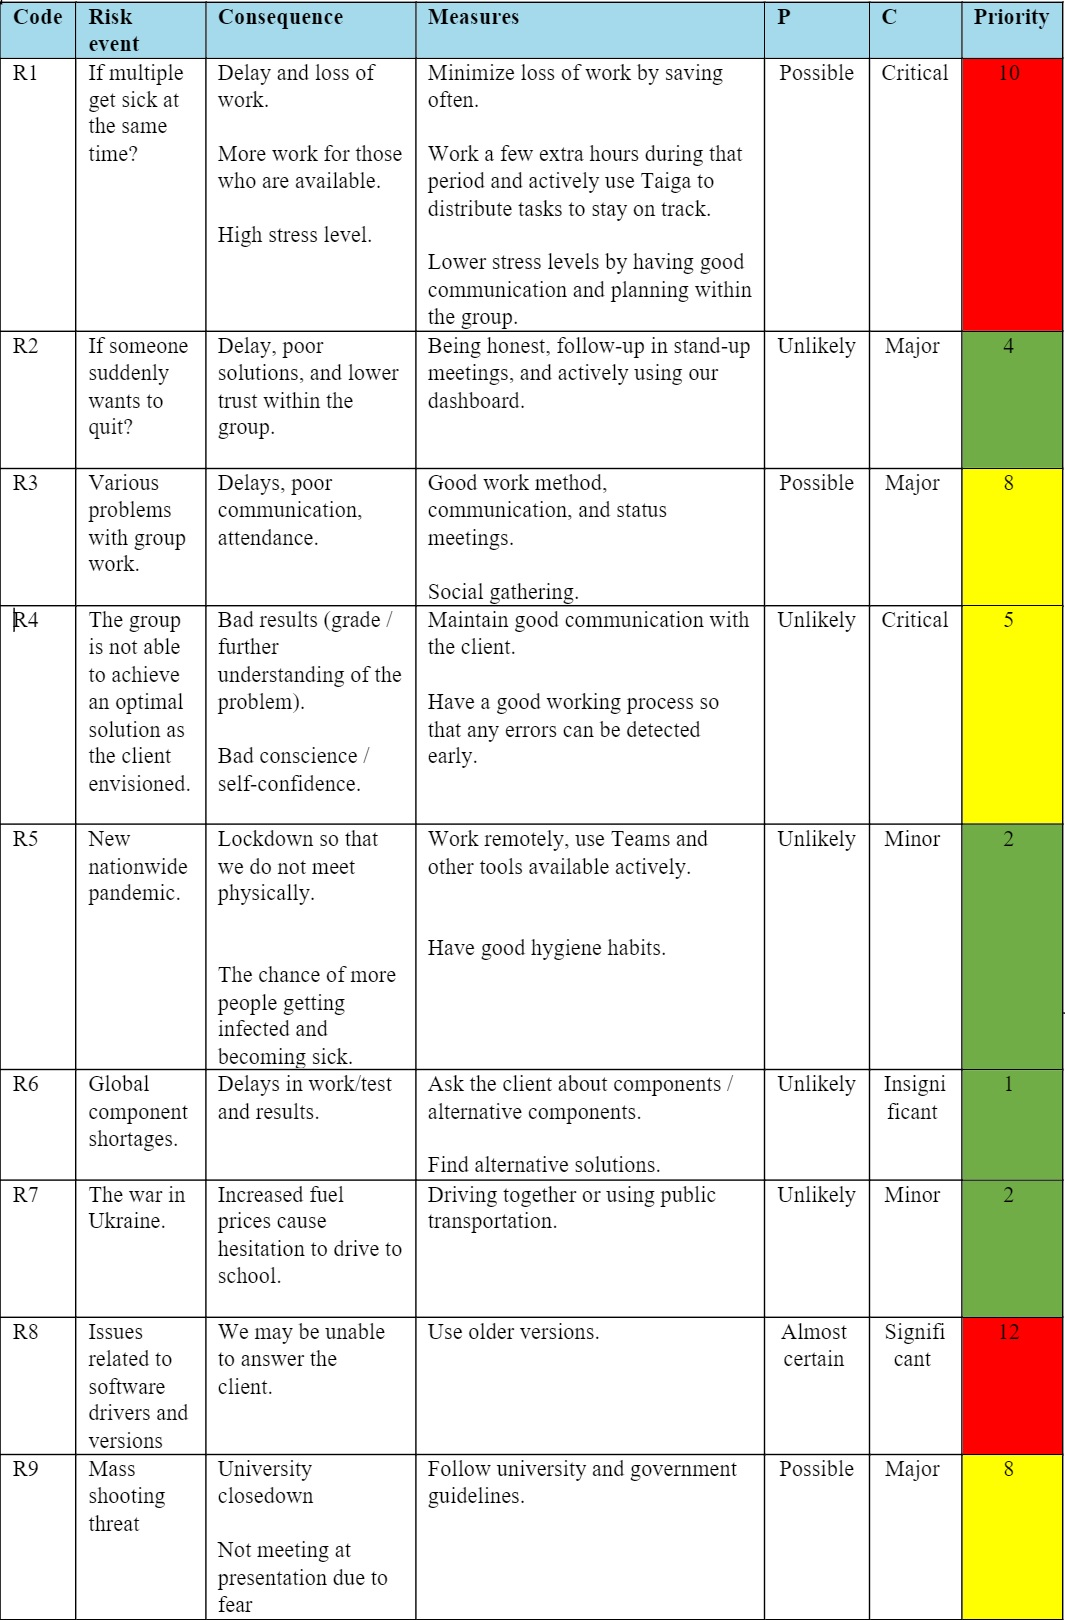
\includegraphics[width=0.85\linewidth]{fig/RisikoTabell.jpg}
\caption{Risk table}
\label{fig:yourlabel}
\end{figure}

\newpage

The prioritization of these risks was determined by evaluating their consequence and probability using the risk matrix:

\begin{figure}[h!]
\centering
\includegraphics[width=0.85\linewidth]{fig/Risk matrix.jpg}
\caption{Risk Matrix \cite{RiskMatrix}} 
\label{fig:yourlabel}
\end{figure}


